\documentclass[conference]{IEEEtran}
\usepackage{cite}
\usepackage{amsmath,amssymb,amsfonts}
\usepackage{algorithmic}
\usepackage{graphicx}
\usepackage{textcomp}
\usepackage{xcolor}
\def\BibTeX{{\rm B\kern-.05em{\sc i\kern-.025em b}\kern-.08em
    T\kern-.1667em\lower.7ex\hbox{E}\kern-.125emX}}
\begin{document}

\title{Portable Visible Spectrophotometer for Glucose Microdroplet Measurements in Digital Microfluidics System}

\author{\IEEEauthorblockN{Alzana Armaniar Farhani}
\IEEEauthorblockA{\textit{School of Electrical Engineering} \\
\textit{and Informatics} \\
\textit{Institut Teknologi Bandung}\\
Bandung, Indonesia \\
Email: farhanialzana@gmail.com}
\and
\IEEEauthorblockN{Balkan Khilmi Assakandari}
\IEEEauthorblockA{\textit{School of Electrical Engineering} \\
\textit{and Informatics} \\
\textit{Institut Teknologi Bandung}\\
Bandung, Indonesia \\
Email: balkankhilmi@gmail.com}
\and
\IEEEauthorblockN{Anindhita Nayazirly}
\IEEEauthorblockA{\textit{School of Electrical Engineering} \\
\textit{and Informatics} \\
\textit{Institut Teknologi Bandung}\\
Bandung, Indonesia \\
Email: zirlysukarno@gmail.com}
\and
\IEEEauthorblockN{Akhmadi Surawijaya}
\IEEEauthorblockA{\textit{School of Electrical Engineering and Informatics} \\
\textit{Institut Teknologi Bandung}\\
Bandung, Indonesia \\
Email:}
\and
\IEEEauthorblockN{Muhammad Ogin Hasanuddin}
\IEEEauthorblockA{\textit{School of Electrical Engineering and Informatics} \\
\textit{Institut Teknologi Bandung}\\
Bandung, Indonesia \\
Email:}
}

\maketitle

\begin{abstract}
    Instrumen yang telah dikembangkan kelompok Tugas Akhir Teknik Elektro sebelumnya adalah sebuah spektrofotometer portabel yang dapat bekerja pada spektrum gelombang ultraviolet dan cahaya tampak, atau umumnya disebut spektrofotometer UV-Vis. Spektrofotometer yang dibuat hanya dapat melakukan perhitungan intensitas cahaya secara relatif terhadap nilai intensitas tertinggi yang terukur, tidak dilakukan kalibrasi skala panjang gelombang dan tuning fungsi konversi citra. Hal ini menunjukkan bahwa pengukuran yang dilakukan masih bersifat kualitatif. Spektrofotometer yang telah dikembangkan kelompok Tugas Akhir Teknik Elektro belum memiliki kapabilitas untuk 
\end{abstract}

\begin{IEEEkeywords}
    UV-VIS Spectrophotometry
\end{IEEEkeywords}

% Pendahuluan
\section{Introduction}
Currently, various methods detect and measure glucose concentrations in food matrices. These methods can be broadly grouped into two main categories: enzymatic approaches, such as spectrophotometric assays; and non-enzymatic instrumentation, such as HPLC systems. While the first group is glucose specific, the latter is broadly adaptable and can be used to detect not only glucose but a wide variety of other carbohydrates as well. However, the spectrophotometric test is becoming a more commonly used method for glucose detection because of its ability to detect in a shorter time and at a lower cost. Spectrophotometric tests utilize the light transmitted or reflected by a sample to perform qualitative and quantitative analysis. For qualitative analysis, the light transmitted by a sample has a unique spectrum based on the atoms or molecules contained in the sample.  

Meanwhile, for quantitative analysis, the absorbance level of the sample for a specific wavelength is directly proportional to the concentration of the sample. Glucose spectrophotometry test includes colorimetric measurement methods, namely measurements that involve changing the color of the sample to measure quantities such as absorbance and sample concentration. Various colorimetric methods involving reactions with different enzymes for glucose measurement are the object of research being developed to obtain colorimetric methods that are accurate, sensitive, selective, and inexpensive.  Several approaches were studied to develop a colorimetric glucose biosensor by using glucose oxidase (GOx) to oxidize glucose to gluconic acid and hydrogen peroxide (H2O2). In colorimetric assays, studies revealed that the Horseradish Peroxidase (HRP) enzyme could catalyze the reaction of H2O2 and organic substrates such as 3,3',5,5'-tetramethylbenzidine (TMB) to produce visible colors[1]. 

Microfluidics offer several advantages for glucose analysis, such as reduced sample and reagent consumption, faster analysis, portability, and high compatibility with multiplexing detection means. One application called digital microfluidics (DMF) has a promising potential to operate microdroplets in portable analytical systems. The platform is based on the droplet manipulation using electrowetting-on-dielectric (EWOD) principle which applies electric potential to the control electrodes coated with a hydrophobic dielectric[2]. The DMF system mainly consists of a fluid layer located between the top and bottom plates. Nowadays, DMF technology is commonly used for various processes which include sample preparation and diagnostics[3]. Droplet mixing allows all chemical reactions to be done on chip. An optical detection system needs to be developed in order to measure the absorbance and concentration of a glucose droplet on the DMF chip. 

In this study, we present the development of a portable visible spectrophotometer, which is detachable to DMF platforms. It allows the integration with a DMF platform and can be removed if the DMF is needed for other purposes. A light will be emitted through the droplet located on the DMF chip and an array of photodetectors will collect the intensity of incident light. A program is uploaded to the system to compute the absorbance and the concentration of the sample droplet. Users can interact with the system using four input buttons and an LCD which displays the result of the measurements. 

The current version of the spectrophotometer has some features as follows:
\begin{itemize}
    \item Concentration measurement of microdroplet samples 
    \item Absorbance measurement of samples based on wavelength characteristic 
    \item Able to work in visible spectrum (400 nm to 700 nm) 
    \item Able to be integrated with a digital microfluidic platform 
    \item The measurement results can be displayed on an LCD and stored 
    \item Portable (12cm x 13cm x 20cm)
\end{itemize}

\section{Methods}
\subsection{System Overview}
The proposed system consists of five subsystems which are light source, light sensor, control, user interface, and power subsystem. Its data flow diagram (DFD) can be seen in Fig. 1. The light sensor subsystem is composed of a slit, a monochromator, and an array of photodetector. The source light, which is emitted by a polychromatic light source, will be passed through the sample droplet located on an electrode of a DMF platform. The light which is not absorbed by the droplet will pass through the slit then to a monochromator. The monochromator decomposes the light into monochromatic light to be detected by the photodetector array. Each detector in the array measures the light intensity for a specific wavelength. The measurement readings will be sent to the control subsystem to be computed into absorbance values. 

    \begin{figure}[htbp]
    \centerline{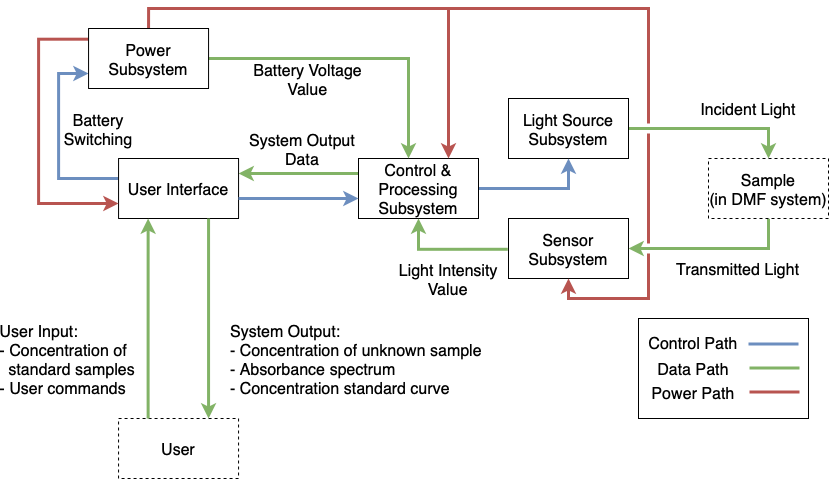
\includegraphics{system-dfd.png}}
    \caption{Level-1 Data Flow Diagram (DFD) of the system.}
    \label{system-dfd}
    \end{figure}

\subsection{Light Source Subsystem}
The light source subsystem functions to produce polychromatic light as the primary variable to be manipulated and measured by the instrument. This subsystem includes 2 modules, namely switching circuits and light sources. The process in this subsystem begins with receiving a control signal from the control subsystem to the switching circuit. The switching circuit then flows the source voltage to the lamp so that it can be lit. The polychromatic light source will illuminate and produce light with all UV-Vis frequencies within the specification. This light is then passed on to the sample for a certain period.

    \begin{figure}[htbp]
    \centerline{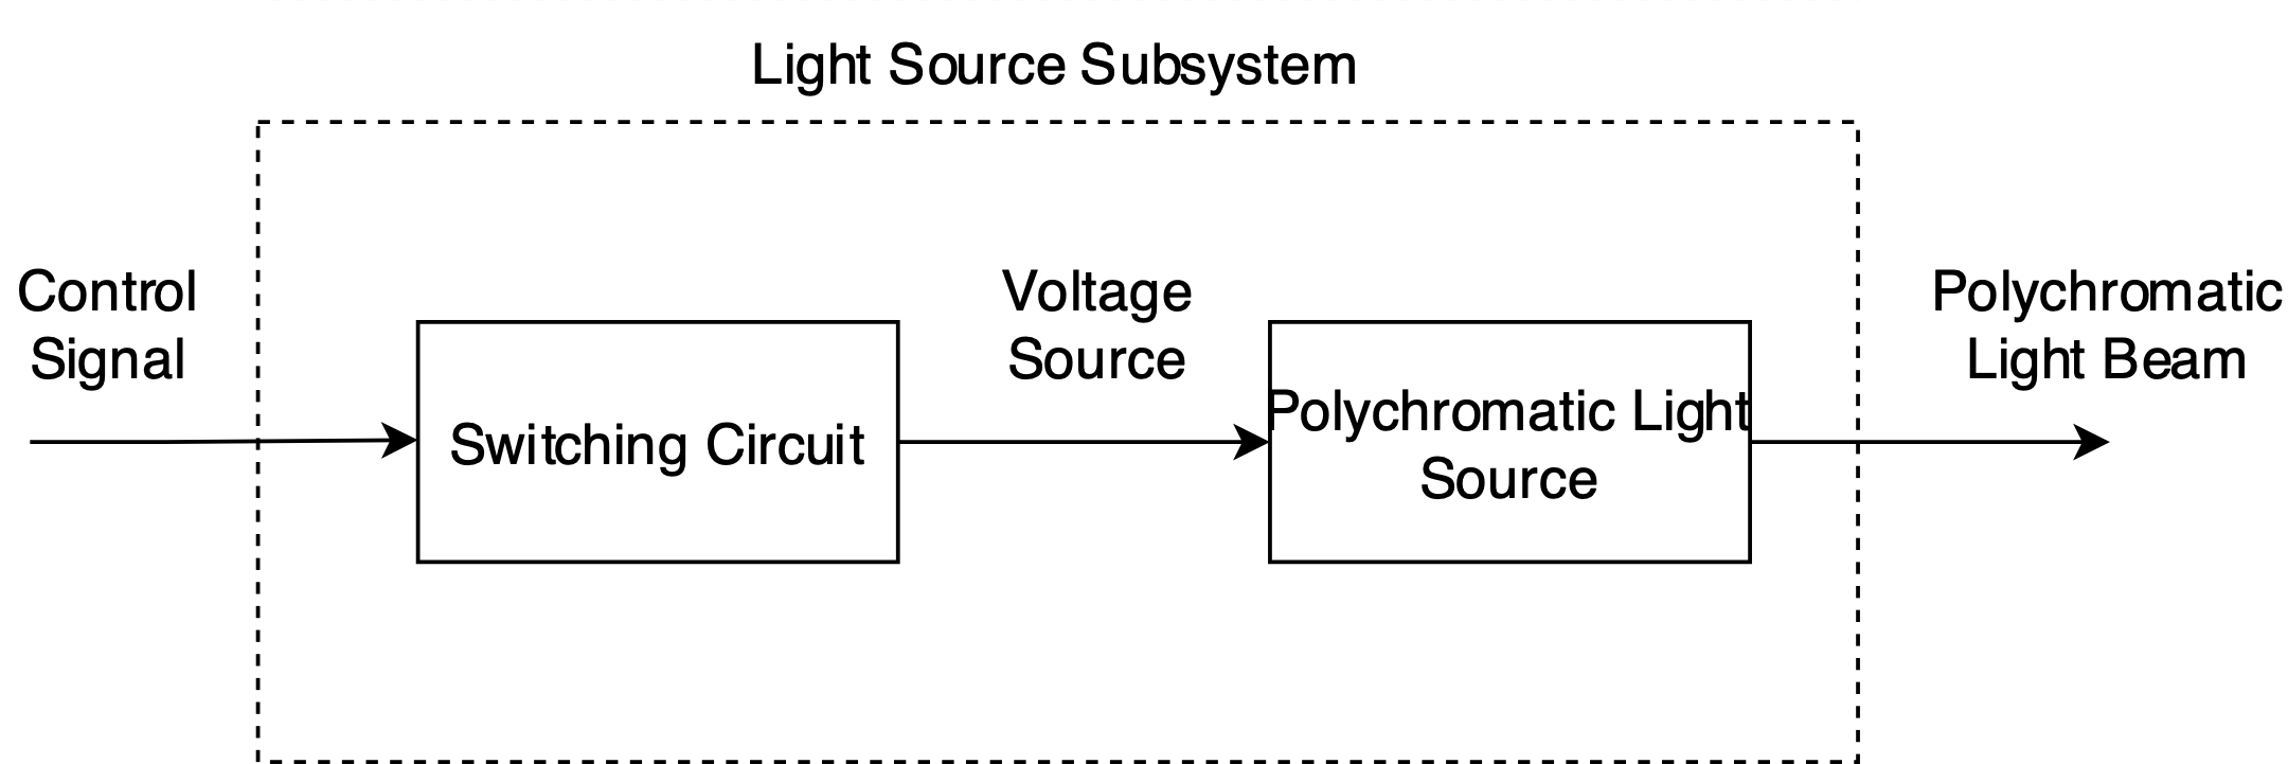
\includegraphics{light-source-dfd.png}}
    \caption{DFD of the light source subsystem.}
    \label{light-source-dfd}
    \end{figure}

\subsection{Light Sensor Subsystem}
The light sensor subsystem functions as a spectrometer that receives polychromatic light beam and outputs light intensities of discrete wavelengths in the form of digital data.
Polychromatic light beam enters the sensor subsystem through a hole and gets diffracted by a transmissive diffraction grating as to spatially separate light by its wavelengths.
The grating has a groove density of 1200 lines per millimeter, thus only the first order of diffraction is usable to separate the visible spectrum.
The resulting ray is then recorded by Micron® Imaging MT9M001 Monochrome CMOS digital image sensor.
Different pixel of the image sensor captures the intensity of different wavelengths ranging from 400 nanometer to 700 nanometer formatted into 10-bit unsigned integer.
The light sensor subsystem outputs, at maximum, 1280 16-bit unsigned integer values, each value representing the light intensity of certain wavelengths. 

    \begin{figure}[htbp]
    \centerline{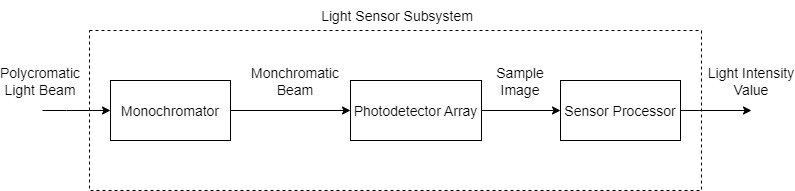
\includegraphics{light-sensor-dfd.png}}
    \caption{DFD of the light sensor subsystem.}
    \label{light-sensor-dfd}
    \end{figure}

\subsection{Control Subsystem}
The subsystems in the spectrophotometer are controlled by a ESP32-S3-WROOM-1-N8 microcontroller module (Espressif Systems, Shanghai, China). The task of the control subsystem is to execute the main workflow of the spectrophotometer by a FSM. The control subsystem synchronizes other subsystems, such as the light source with the light sensor when measuring light intensities. The subsystem also has non-volatile memory storage to save past absorbance measurements and concentration calibration curves.

    \begin{figure}[htbp]
    \centerline{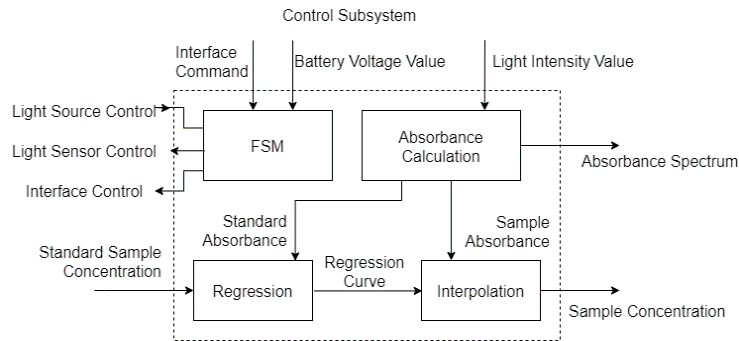
\includegraphics{control-dfd.png}}
    \caption{DFD of the control subsystem.}
    \label{control-dfd}
    \end{figure}

\subsection{User Interface Subsystem}
The user interface subsystem plays a role in connecting the system and the users. This can be done by interpreting the commands given by users through the input interface devices and process it into control signals that will be sent to the control subsystem. The subsystem also has a function to display measurement data which include sample concentration values, sample absorbance spectrum, regression curves, menus, and settings. Fig. 5 shows the data flow diagram of the user interface subsystem.

Four push buttons and a power switch are used as the input interface devices. For the display, a 3.5-inch non-touchscreen TFT LCD with ILI9488 driver is used. The configuration of buttons and non-touchscreen LCD is chosen because it fits the users who use the spectrophotometer using laboratory gloves.

    \begin{figure}[htbp]
    \centerline{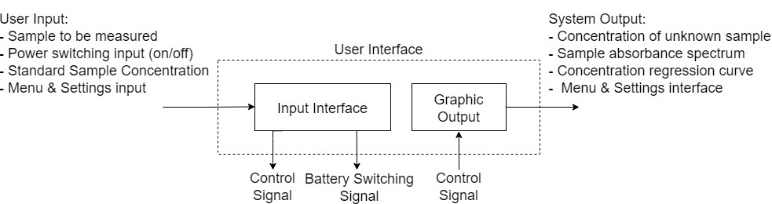
\includegraphics{ui-dfd.png}}
    \caption{DFD of the user interface subsystem.}
    \label{ui-dfd}
    \end{figure}


\subsection{Power Subsystem}
The power subsystem enables the system to be activated by supplying power from the battery to the entire electrical circuit. The battery can be recharged easily whenever the battery voltage is insufficient. The power subsystem also provides information about the battery voltage value to be displayed to the user. 

The power subsystem is activated when the user presses the power button for the first time—allowing the power to flow to the microcontroller. The microcontroller will supply power to certain sub-blocks according to user input by adjusting the whether the battery voltage is sufficient based on a specified threshold. If the battery voltage value is below the threshold or the user presses the power button again, the power supply to the entire circuit will be cut off, and the system will be disabled.

    \begin{figure}[htbp]
    \centerline{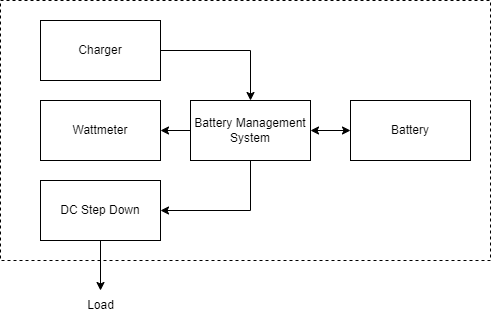
\includegraphics{power-dfd.png}}
    \caption{DFD of the power subsystem.}
    \label{power-dfd}
    \end{figure}

% Pendahuluan
\section{Results and Discussion}
\subsection{Accuracy}
\subsection{Repeatability}
\subsection{Wavelength Range}
\subsection{Device and DMF Cartridge Distance}
\subsection{Electronic Display Size}
\subsection{Weight and Size}

\section{Conclusions}

\section*{References}


\begin{thebibliography}{00}
\bibitem{b1} H. V. Tran et al., “Silver nanoparticles-decorated reduced graphene oxide: A novel peroxidase-like activity nanomaterial for development of a colorimetric glucose biosensor,” Arabian Journal of Chemistry, vol. 13, no. 7, pp. 6084–6091, Jul. 2020, doi: 10.1016/j.arabjc.2020.05.008.
\bibitem{b2} Z. Gu, M. L. Wu, B. Y. Yan, H. F. Wang, and C. Kong, “Integrated Digital Microfluidic Platform for Colorimetric Sensing of Nitrite,” ACS Omega, vol. 5, no. 19, pp. 11196–11201, May 2020, doi: 10.1021/acsomega.0c01274.
\bibitem{b3} S. Huang and R. B. Fair, “Quantitative measurements of inorganic analytes on a digital microfluidics platform,” SN Applied Sciences, vol. 1, no. 12, Dec. 2019, doi: 10.1007/s42452-019-1693-8.
\end{thebibliography}

\end{document}